\documentclass[12pt]{article}
\usepackage[T1]{fontenc}
\usepackage[light,math]{iwona}
\usepackage[latin1]{inputenc}
\usepackage{amsmath}
\usepackage{mathtools}
\usepackage{xspace}
\usepackage{graphicx}
\usepackage[english]{babel}
\usepackage[font=small,labelfont=bf]{caption}
\usepackage[centering,includeheadfoot,margin=2cm]{geometry}
\usepackage{tikz}
\usetikzlibrary{shapes,arrows,automata,trees, shadows,decorations.pathmorphing}
\title{CS375 WK5}
\author{Jason N Mansfield}
\begin{document}

\begin{figure}
\begin{center}
\caption{Q01: $L_1$ = (a+b)*a}
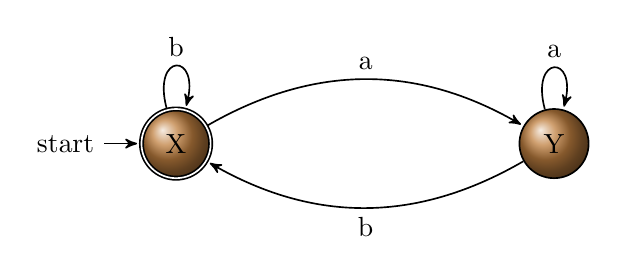
\begin{tikzpicture}[->,>=stealth',shorten >=1pt,auto,node distance=4.8cm, semithick]
\tikzstyle{every state}=[draw=black,text=black, ball color=brown]
\node[initial,state,accepting] (X) {X};
\node[state][right of=X](Y){Y};
\path (Y)edge [bend left] node{b}(X)
         edge  [loop above]node{a}(Y)
         (X)edge [loop above]node{b}(X)
         edge [bend left] node{a}(Y);
\end{tikzpicture} 
\end{center}
\end{figure}

\begin{figure}
\begin{center}
\caption{Q01: $L_2$= b(a+b)*}
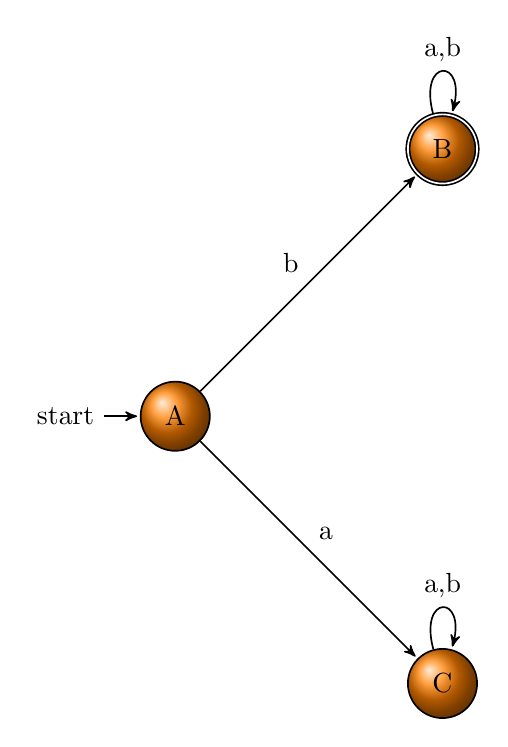
\begin{tikzpicture}[->,>=stealth',shorten >=1pt,auto,node distance=4.8cm, semithick]
\tikzstyle{every state}=[draw=black,text=black, ball color=orange]
\node[initial,state] (A) {A};
\node[state,accepting][above right of=A](B){B};
\node[state][below right of=A](C){C};
\path (A)edge node{b}(B)
         edge  node{a}(C)
      (B)edge  [loop above]node{a,b}(B)
      (C)edge [loop above]node{a,b}(C);
\end{tikzpicture} 
\end{center}
\end{figure}


\begin{figure}
\begin{center}
\caption{Q01: $L_1$$\bigcap$$L_2$}
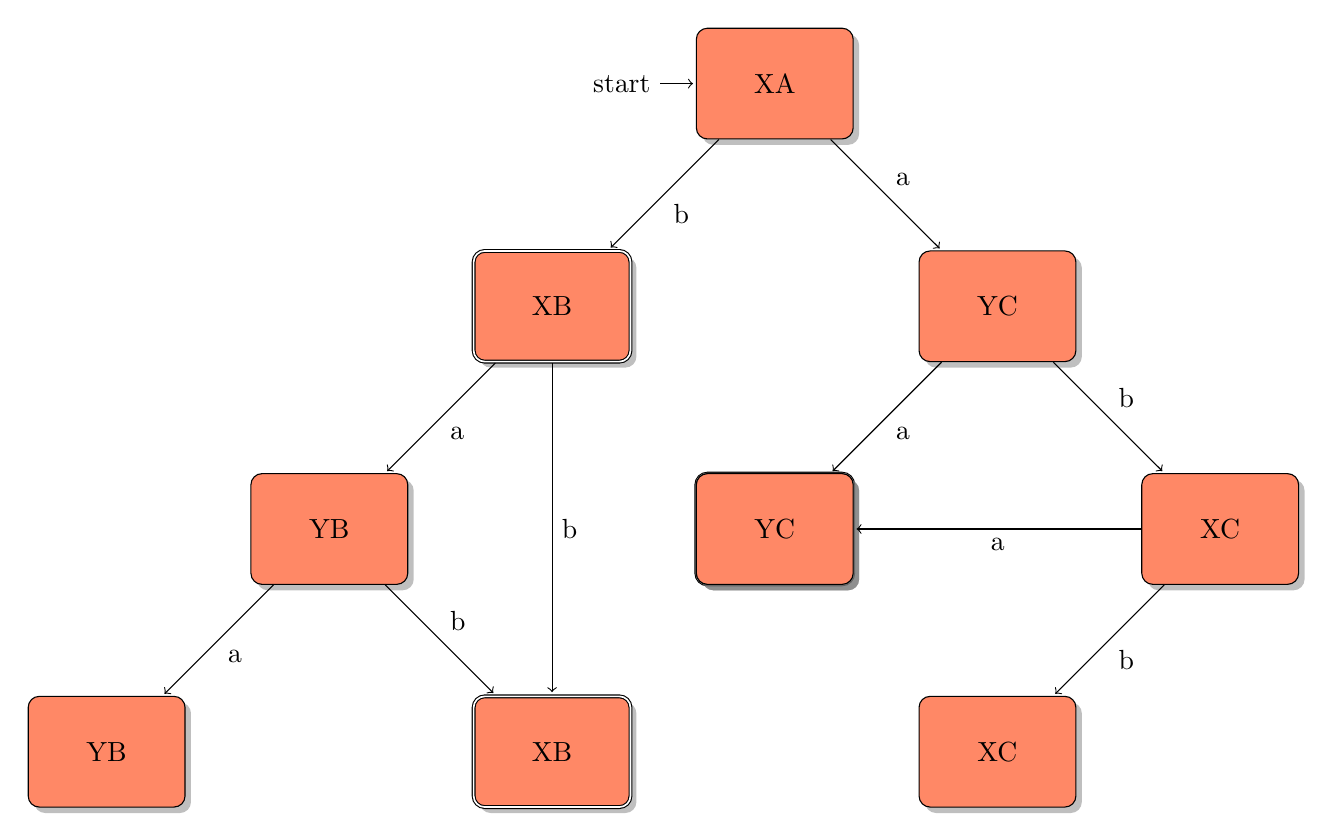
\begin{tikzpicture}[->,shorten >=1pt,node distance=4cm,auto]
\tikzstyle{every state} = [rectangle, draw, fill=orange!45!red!60!, text width=5em, text centered, rounded corners, minimum height=4em, drop shadow]
\node[initial,state] (XA){XA};
\node[state,accepting][below left of=XA](XB){XB};
\node[state,accepting][below right of=XB](XB2){XB};
\node[state][below left of=XB](YB){YB};
\node[state,accepting][below right of=YB](XB3){XB};
\node[state][below left of=YB](YB2){YB};
\node[state][below right of=XA](YC){YC};
\node[state][below left of=YC](YC2){YC};
\node[state][below left of=YC](YC3){YC};
\node[state](XC)[below right of=YC]{XC};
\node[state](XC2)[below left of=XC]{XC};
\path (XA)edge node{b}(XB)
                edge node{a}(YC)
          (YC)edge node{a}(YC2)
                edge node{b}(XC)
          (XC)edge node{a}(YC3)
                edge node{b}(XC2)
          (XB)edge node{a}(YB)
                edge node{b}(XB3)
          (YB)edge node{a}(YB2)
                edge node{b}(XB3);
\end{tikzpicture}
\end{center}
\end{figure}

\begin{figure}
\begin{center}
\caption{Q01: $L_3$ = b(b+aa*b)*}
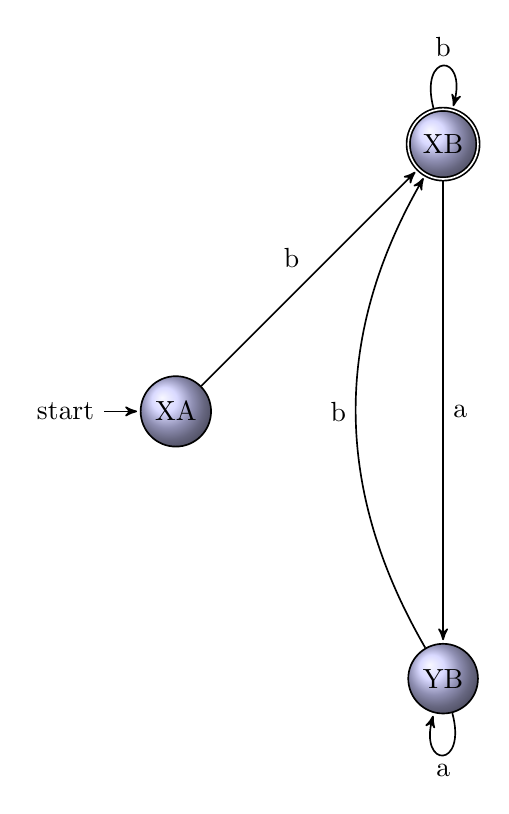
\begin{tikzpicture}[->,>=stealth',shorten >=1pt,auto,node distance=4.8cm, semithick]
\tikzstyle{every state}=[draw=black,text=black, ball color=blue!20]
\node[initial,state] (XA) {XA};
\node[state,accepting][above right of=XA](XB){XB};
\node[state][below right of=XA](YB){YB};
\path (XA)edge node{b}(XB)
         (XB)edge  [loop above]node{b}(XB)
               edge node{a}(YB)
         (YB)edge [loop below]node{a}(YB)
               edge [bend left]node{b}(XB);
\end{tikzpicture} 
\end{center}
\end{figure}
\clearpage

\begin{figure}
\begin{center}
\caption{Q02: $L_1$ = (a+b)b(a+b)*}
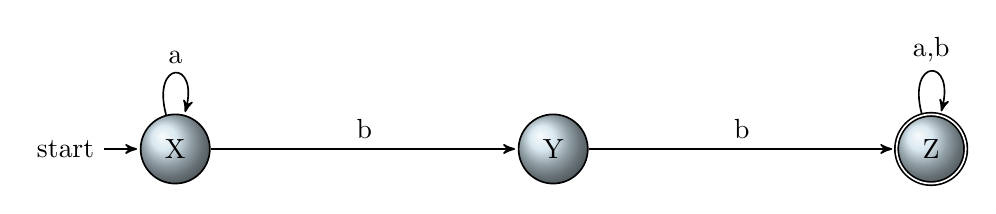
\begin{tikzpicture}[->,>=stealth',shorten >=1pt,auto,node distance=4.8cm, semithick]
\tikzstyle{every state}=[draw=black,text=black, ball color=green!40!blue!20!]
\node[initial,state] (X) {X};
\node[state] [right of=X](Y){Y};
\node[state,accepting][right of=Y](Z){Z};
\path (X)edge [loop above]node{a}(X)
              edge node{b}(Y)
              (Y)edge node{b}(Z)
          (Z)edge [loop above]node{a,b}(Z);   
\end{tikzpicture} 
\end{center}
\end{figure}

\begin{figure}
\begin{center}
\caption{Q02: $L_2$= b(a+b)*}
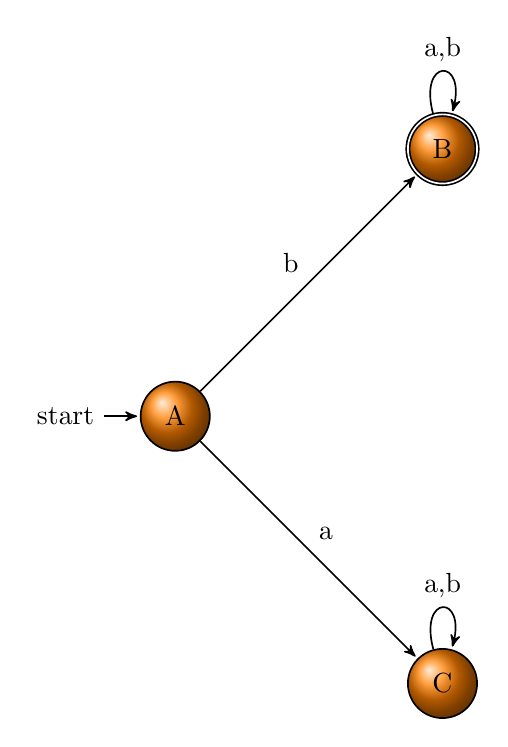
\begin{tikzpicture}[->,>=stealth',shorten >=1pt,auto,node distance=4.8cm, semithick]
\tikzstyle{every state}=[draw=black,text=black, ball color=orange]
\node[initial,state] (A) {A};
\node[state,accepting][above right of=A](B){B};
\node[state][below right of=A](C){C};
\path (A)edge node{b}(B)
         edge  node{a}(C)
      (B)edge  [loop above]node{a,b}(B)
      (C)edge [loop above]node{a,b}(C);
\end{tikzpicture} 
\end{center}
\end{figure}

\begin{figure}
\begin{center}
\caption{Q02: $L_1$$\bigcap$$L_2$}
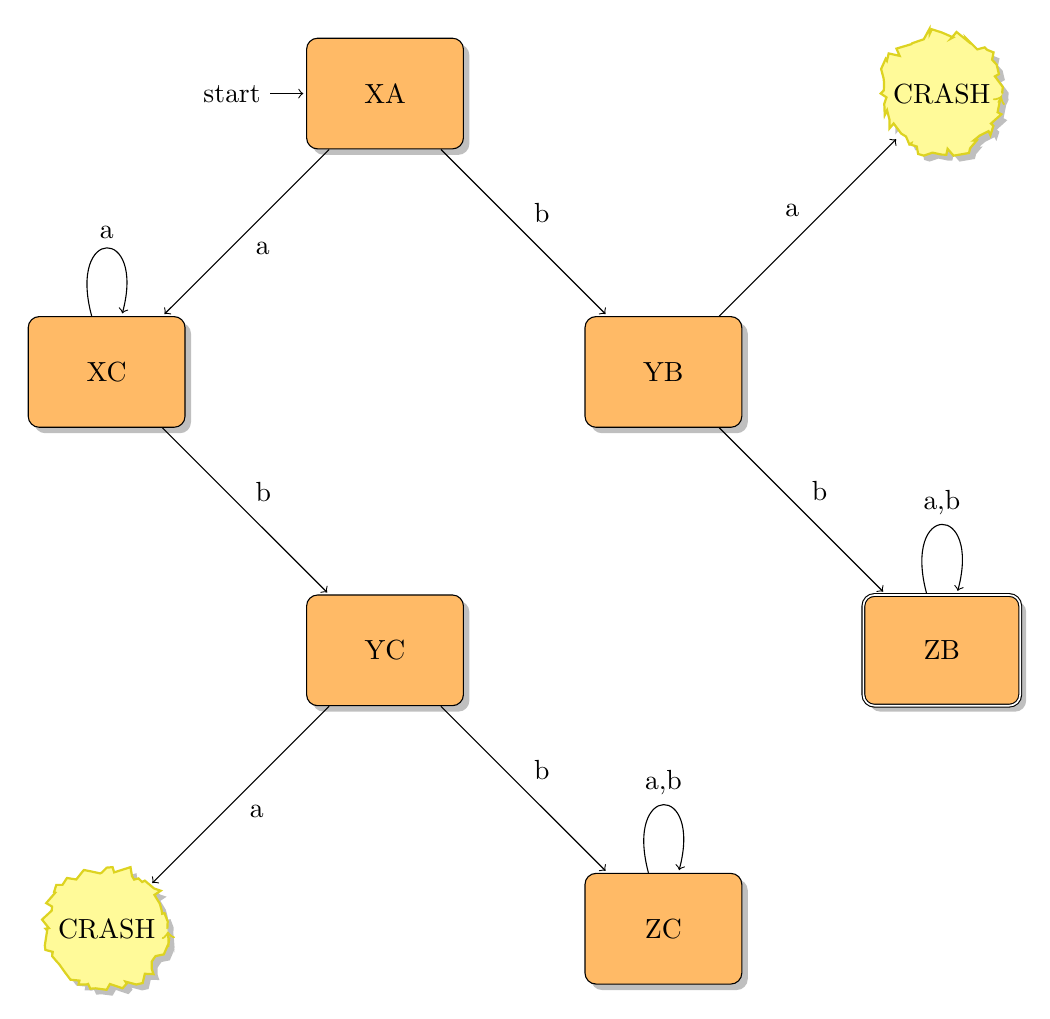
\begin{tikzpicture}[->,shorten >=1pt,node distance=5cm,auto]
\tikzstyle{every state} = [rectangle, draw, fill=red!45!yellow!60!, text width=5em, text centered, rounded corners, minimum height=4em, drop shadow]
\tikzstyle{noise}=[circle,
                                    thick,
                                    minimum size=1.2cm,
                                    draw=yellow!85!black,
                                    fill=yellow!40,
                                    decorate,
                                    drop shadow,
                                    decoration={random steps,
                                                            segment length=2pt,
                                                            amplitude=2pt}]
\node[initial,state] (XA){XA};
\node[state][below left of=XA](XC){XC};
\node[state][below right of=XC](YC){YC};
\node[state][below right of=YC](ZC){ZC};
\node[noise][below left of=YC](CRASH){CRASH};
\node[state][below right of=XA](YB){YB};
\node[noise][above right of=YB](CRASH2){CRASH};
\node[state, accepting][below right of=YB](ZB){ZB};
\path (XA)edge node{a}(XC)
                edge node{b}(YB)
          (XC)edge [loop above]node{a}(XC)
                edge node{b}(YC)
          (YC)edge node{a}(CRASH)
                edge node{b}(ZC)
          (ZC)edge [loop above] node{a,b}(ZC)
          (ZB)edge [loop above]node{a,b}(ZB)
          (YB)edge node{a}(CRASH2)
                edge node{b}(ZB);
\end{tikzpicture}
\end{center}
\end{figure}

\begin{figure}
\begin{center}
\caption{Q02: $L_3$ = ab(a+b)*}
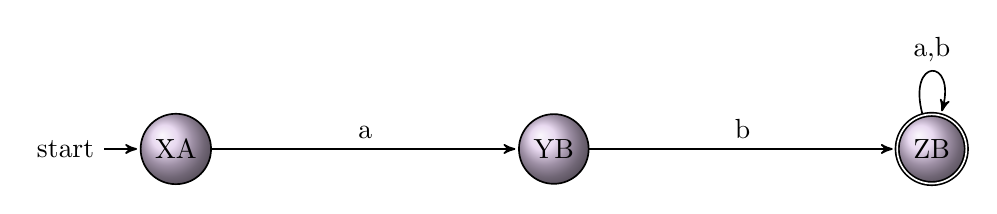
\begin{tikzpicture}[->,>=stealth',shorten >=1pt,auto,node distance=4.8cm, semithick]
\tikzstyle{every state}=[draw=black,text=black, ball color=red!40!blue!20!]
\node[initial,state] (XA) {XA};
\node[state] [right of=XA](YB){YB};
\node[state,accepting][right of=YB](ZB){ZB};
\path (XA)edge node{a}(YB)
          (YB)edge node{b}(ZB)
          (ZB)edge [loop above]node{a,b}(ZB); 
\end{tikzpicture} 
\end{center}
\end{figure}

\begin{figure}
\begin{center}
\caption{Q03: $L_1$ = (b+ab)*(a+$\Lambda$)}
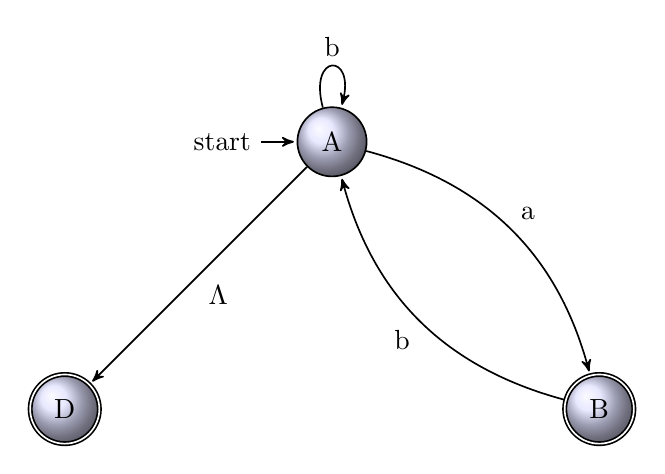
\begin{tikzpicture}[->,>=stealth',shorten >=1pt,auto,node distance=4.8cm, semithick]
\tikzstyle{every state}=[draw=black,text=black, ball color=white!40!blue!20!]
\node[initial,state] (A) {A};
\node[state,accepting] [below right of=A](B){B};
\node[state,accepting][below left of=A](D){D};
\path (A)edge [bend left]node{a}(B)
              edge [loop above]node{b}(A)
              edge node{$\Lambda$}(D)
          (B)edge [bend left]node{b}(A);
            
             
\end{tikzpicture} 
\end{center}
\end{figure}

\begin{figure}
\begin{center}
\caption{Q03: $L_2$ = (a+b)*aa(a+b)*}
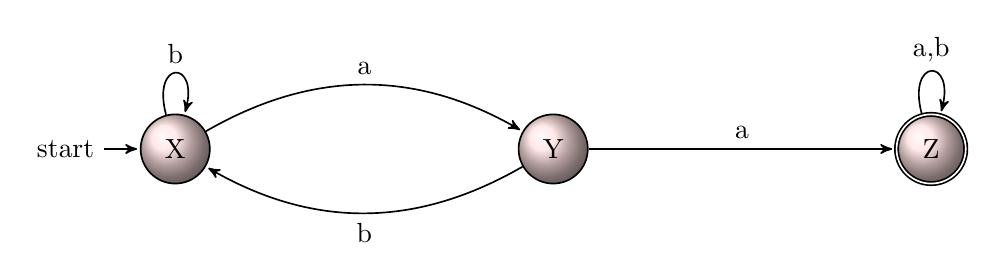
\begin{tikzpicture}[->,>=stealth',shorten >=1pt,auto,node distance=4.8cm, semithick]
\tikzstyle{every state}=[draw=black,text=black, ball color=white!40!red!20!]
\node[initial,state] (X) {X};
\node[state][right of=X](Y){Y};
\node[state,accepting][right of=Y](Z){Z};
\path (X)edge [bend left]node{a}(Y)
              edge[loop above]node{b}(X)
         (Y)edge node{a}(Z)
              edge [bend left]node{b}(X)
         (Z)edge [loop above]node{a,b}(Z);
\end{tikzpicture} 
\end{center}
\end{figure}

\begin{figure}
\begin{center}
\caption{Q02: $L_1$$\bigcap$$L_2$}
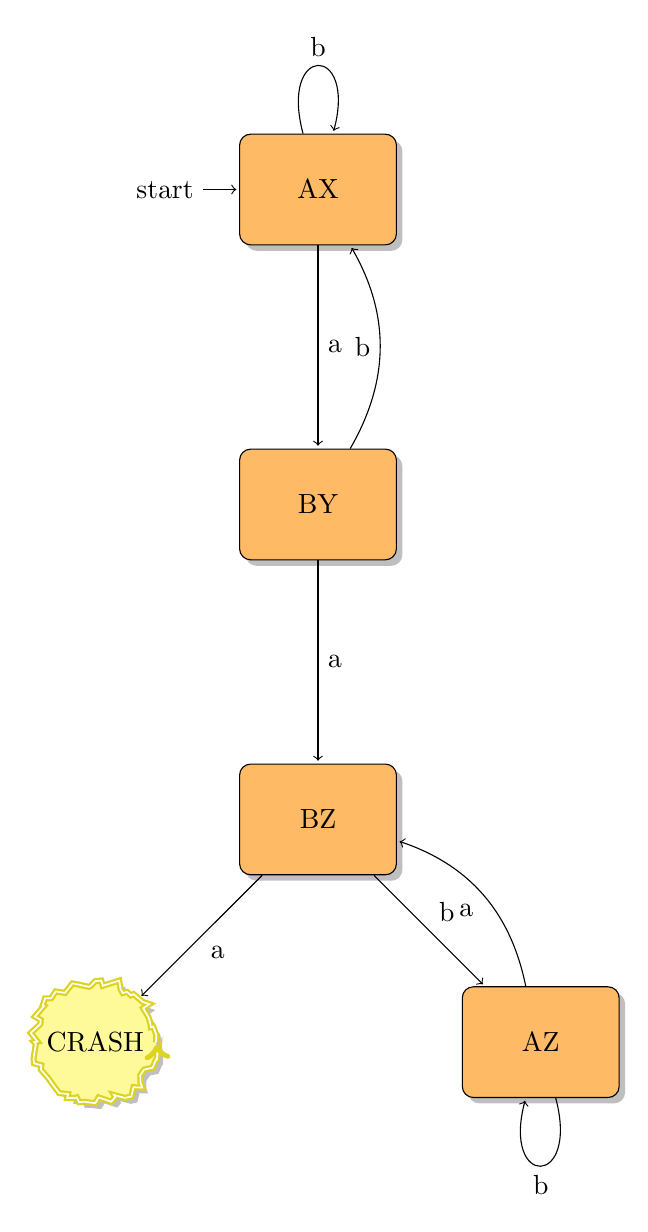
\begin{tikzpicture}[->,shorten >=1pt,node distance=4cm,auto]
\tikzstyle{every state} = [rectangle, draw, fill=red!45!yellow!60!, text width=5em, text centered, rounded corners, minimum height=4em, drop shadow]
\tikzstyle{noise}=[circle,
                                    thick,
                                    minimum size=1.2cm,
                                    draw=yellow!85!black,
                                    fill=yellow!40,
                                    decorate,
                                    drop shadow,
                                    decoration={random steps,
                                                            segment length=2pt,
                                                            amplitude=2pt}]
\node[initial,state] (AX){AX};
\node[state][below of=AX](BY){BY};
\node[state][below of=BY](BZ){BZ};
\node[noise,accepting][below left of=BZ](CRASH){CRASH};
\node[state][below right of=BZ](AZ){AZ};
\path (AX)edge node{a}(BY)
                edge [loop above]node{b}(AX)
          (BY)edge node{a}(BZ)
                edge [bend right]node{b}(AX)
          (BZ)edge node{b}(AZ)
                edge node{a}(CRASH)
          (AZ)edge [bend right]node{a}(BZ)
                edge [loop below]node{b}(AZ);
         
\end{tikzpicture}
\end{center}
\end{figure}
\begin{figure}
\begin{center}
\caption{Q03: $L_3$ = (b+ab)*aa(bb*a)*}
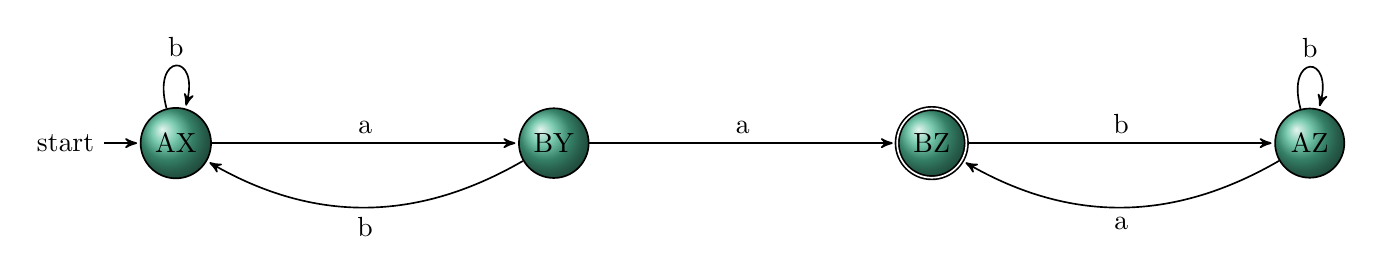
\begin{tikzpicture}[->,>=stealth',shorten >=1pt,auto,node distance=4.8cm, semithick]
\tikzstyle{every state}=[draw=black,text=black, ball color=blue!40!green!70!]
\node[initial,state] (AX) {AX};
\node[state][right of=AX](BY){BY};
\node[state,accepting][right of=BY](BZ){BZ};
\node[state][right of=BZ](AZ){AZ};
\path (AX)edge [loop above]node{b}(AX)
                edge node{a}(BY)
          (BY)edge [bend left]node{b}(AX)
                edge node{a}(BZ)
          (BZ)edge node{b}(AZ)
          (AZ)edge [bend left]node{a}(BZ)
                edge [loop above]node{b}(AZ);   
\end{tikzpicture} 
\end{center}
\end{figure}
\clearpage
\begin{figure}
\begin{center}
\caption{Q04: $L_1$ = (aa+ab+ba+bb)*}
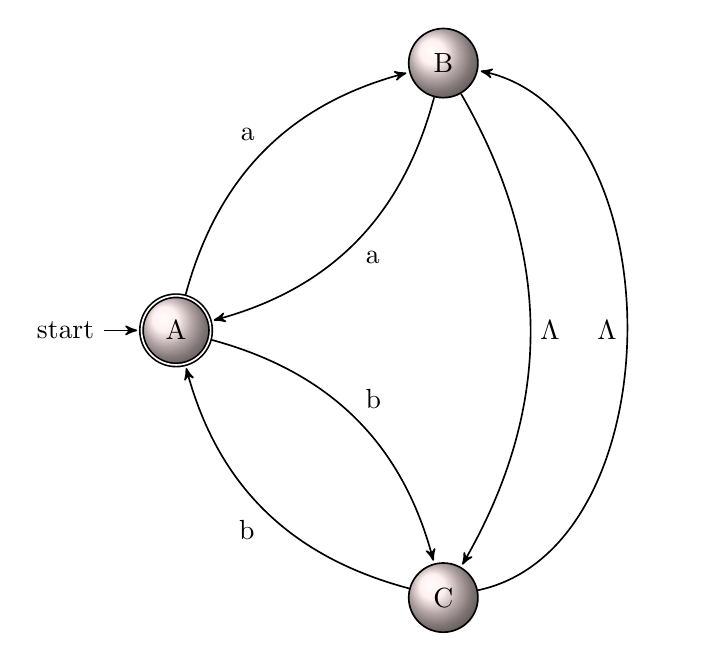
\begin{tikzpicture}[->,>=stealth',shorten >=1pt,auto,node distance=4.8cm, semithick]
\tikzstyle{every state}=[draw=black,text=black, ball color=red!40!white!20!]
\node[initial,state,accepting] (A) {A};
\node[state][above right of=A](B){B};
\node[state][below right of=A](C){C};
\path (A)edge [bend left]node{a}(B)
              edge [bend left]node{b}(C)
          (B)edge [bend left]node{a}(A)
              edge [bend left]node{$\Lambda$}(C)
          (C)edge [bend left]node{b}(A)
              edge [bend right=78]node{$\Lambda$}(B);          
\end{tikzpicture} 
\end{center}
\end{figure}

\begin{figure}
\begin{center}
\caption{Q04: $L_2$= b(a+b)*}
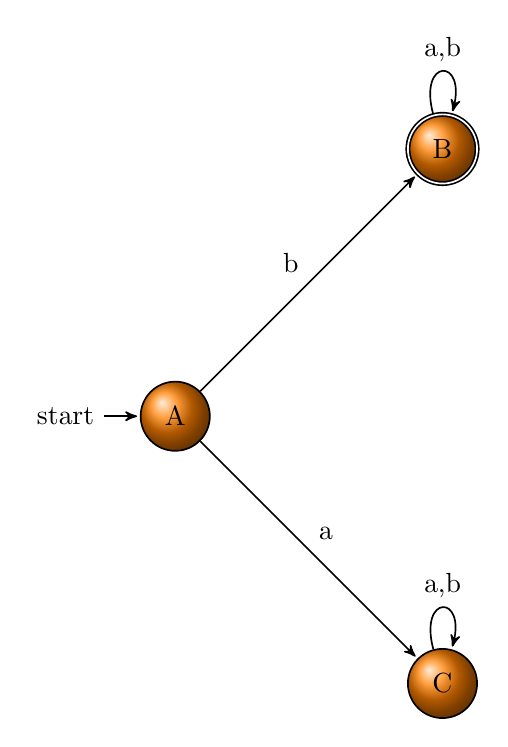
\begin{tikzpicture}[->,>=stealth',shorten >=1pt,auto,node distance=4.8cm, semithick]
\tikzstyle{every state}=[draw=black,text=black, ball color=orange]
\node[initial,state] (A) {A};
\node[state,accepting][above right of=A](B){B};
\node[state][below right of=A](C){C};
\path (A)edge node{b}(B)
         edge  node{a}(C)
      (B)edge  [loop above]node{a,b}(B)
      (C)edge [loop above]node{a,b}(C);
\end{tikzpicture} 
\end{center}
\end{figure}

\begin{figure}
\begin{center}
\caption{Q04: $L_1$$\bigcap$$L_2$}
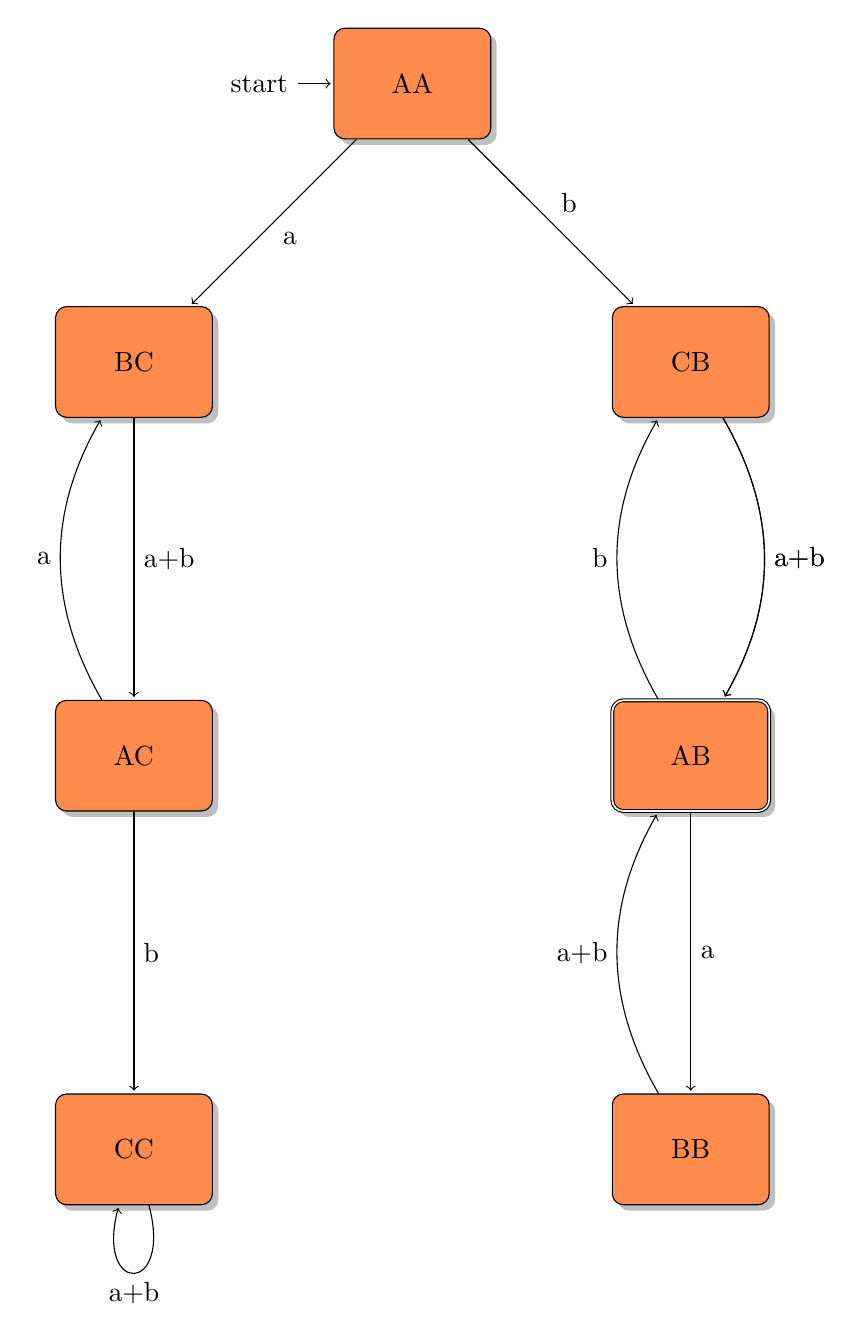
\begin{tikzpicture}[->,shorten >=1pt,node distance=5cm,auto]
\tikzstyle{every state} = [rectangle, draw, fill=red!65!yellow!70!, text width=5em, text centered, rounded corners, minimum height=4em, drop shadow]
\node[initial,state] (AA){AA};
\node[state][below left of=AA](BC){BC};
\node[state][below right of=AA](CB){CB};
\node[state][below of=BC](AC){AC};
\node[state,accepting][below of=CB](AB){AB};
\node[state][below of=AC](CC){CC};
\node[state][below of=AB](BB){BB};
\path (AA)edge node{a}(BC)
                edge node{b}(CB)
          (BC)edge node{a+b}(AC)
          (AC)edge [bend left]node{a}(BC)
                edge node{b}(CC)
          (CC)edge [loop below]node{a+b}(CC)
          (CB)edge [bend left]node{a+b}(AB)
          (AB)edge node{a}(BB)
                edge [bend left]node{b}(CB)
          (BB)edge [bend left]node{a+b}(AB)
          (CB)edge [bend left]node{a+b}(AB);
          
\end{tikzpicture}
\end{center}
\end{figure}

\begin{figure}
\begin{center}
\caption{Q04: $L_3$= b(a+b)(b(a+b)+a(a+b))}
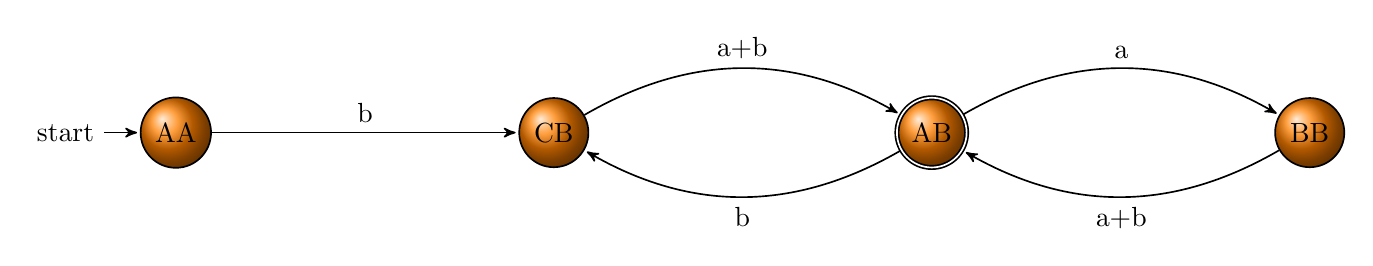
\begin{tikzpicture}[->,>=stealth',shorten >=1pt,auto,node distance=4.8cm, semithick]
\tikzstyle{every state}=[draw=black,text=black, ball color=orange]
\node[initial,state] (AA) {AA};
\node[state][right of=AA](CB){CB};
\node[state,accepting][right of=CB](AB){AB};
\node[state][right of=AB](BB){BB};
\path (AA)edge node{b}(CB)
          (CB)edge [bend left]node{a+b}(AB)
          (AB)edge [bend left]node{b}(CB)
                edge [bend left]node{a}(BB)
          (BB)edge [bend left]node{a+b}(AB);
       
\end{tikzpicture} 
\end{center}
\end{figure}
\clearpage

\begin{figure}
\begin{center}
\caption{Q05: $L_1$ = (aaa+bbb)*}
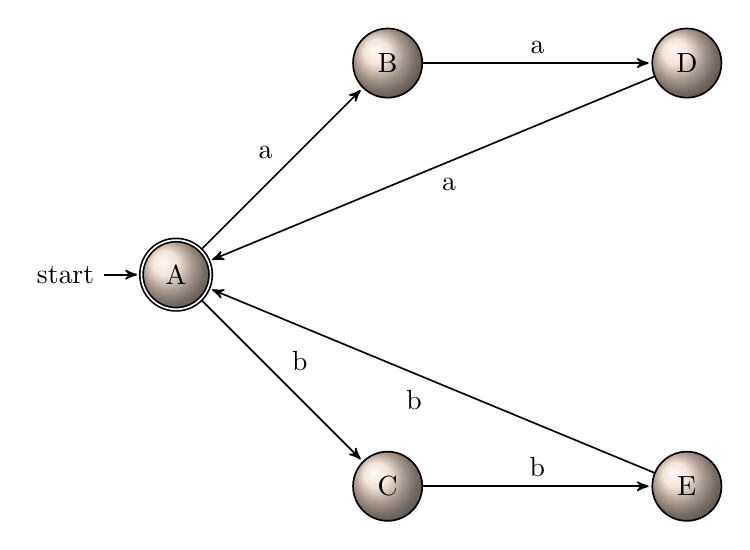
\begin{tikzpicture}[->,>=stealth',shorten >=1pt,auto,node distance=3.8cm, semithick]
\tikzstyle{every state}=[draw=black,text=black, ball color=red!70!green!20!]
\node[initial,state,accepting] (A) {A};
\node[state][above right of=A](B){B};
\node[state][below right of=A](C){C};
\node[state][right of=B](D){D};
\node[state][right of=C](E){E};
\path (A)edge node{a}(B)
              edge node{b}(C)
          (B)edge node{a}(D)
          (D)edge node{a}(A)
          (C)edge node{b}(E)
          (E)edge node{b}(A);    
\end{tikzpicture} 
\end{center}
\end{figure}

\begin{figure}
\begin{center}
\caption{Q05: $L_2$= a(a+b)*}
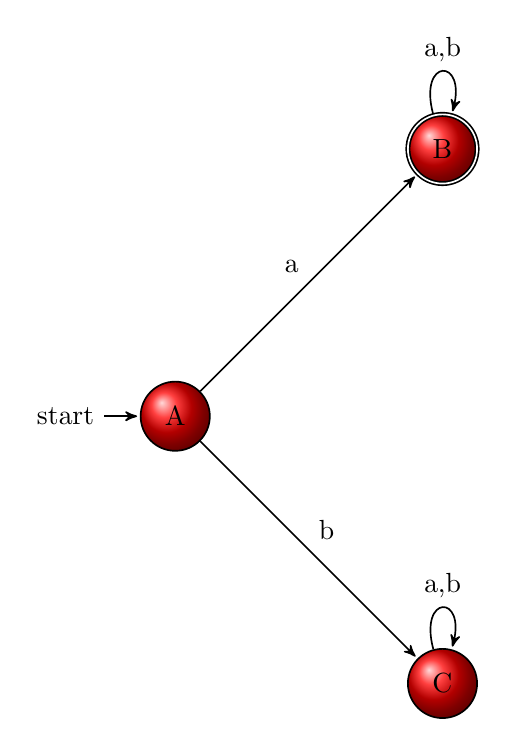
\begin{tikzpicture}[->,>=stealth',shorten >=1pt,auto,node distance=4.8cm, semithick]
\tikzstyle{every state}=[draw=black,text=black, ball color=red]
\node[initial,state] (A) {A};
\node[state,accepting][above right of=A](B){B};
\node[state][below right of=A](C){C};
\path (A)edge node{a}(B)
         edge  node{b}(C)
      (B)edge  [loop above]node{a,b}(B)
      (C)edge [loop above]node{a,b}(C);
\end{tikzpicture} 
\end{center}
\end{figure}

\clearpage
\begin{figure}
\begin{center}
\caption{Q05: $L_1$$\bigcap$$L_2$}
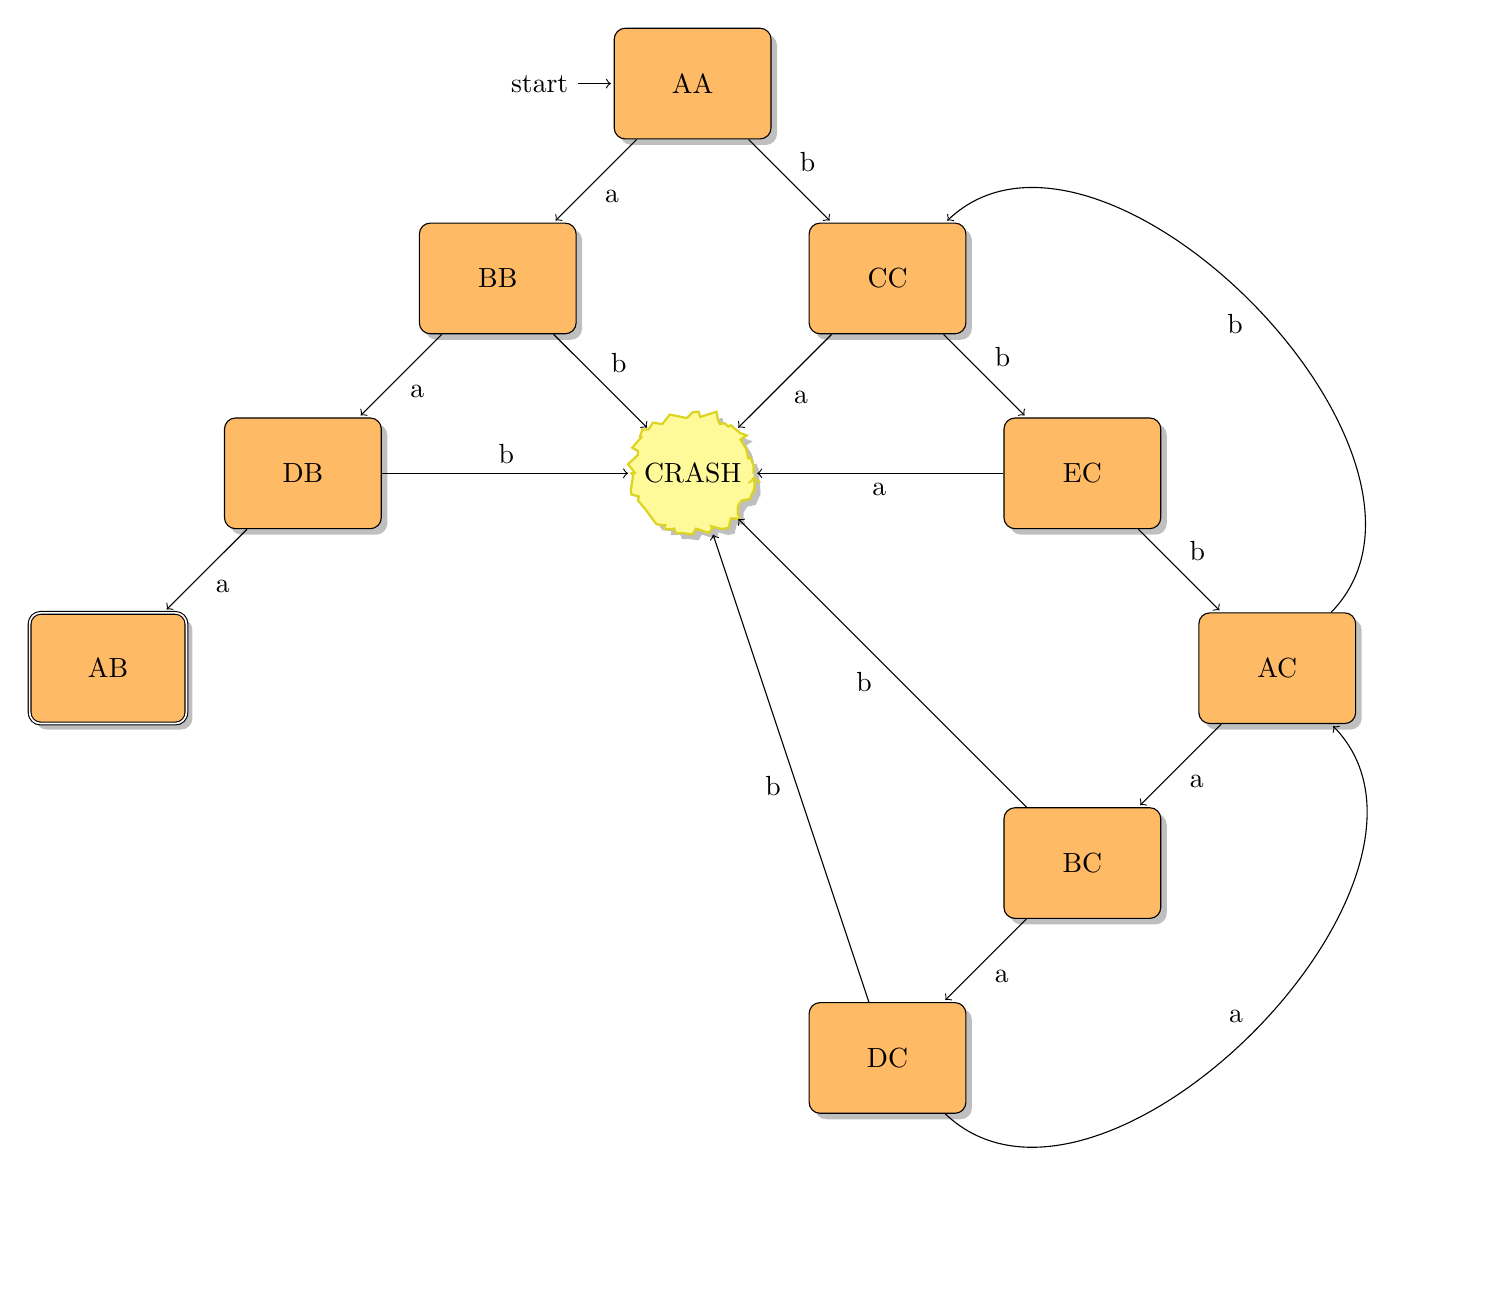
\begin{tikzpicture}[->,shorten >=1pt,node distance=3.5cm,auto]
\tikzstyle{every state} = [rectangle, draw, fill=red!45!yellow!60!, text width=5em, text centered, rounded corners, minimum height=4em, drop shadow]
\tikzstyle{noise}=[circle,
                                    thick,
                                    minimum size=1.2cm,
                                    draw=yellow!85!black,
                                    fill=yellow!40,
                                    decorate,
                                    drop shadow,
                                    decoration={random steps,
                                                            segment length=2pt,
                                                            amplitude=2pt}]
\node[initial,state] (AA){AA};
\node[state][below left of=AA](BB){BB};
\node[state][below left of=BB](DB){DB};
\node[noise][below right of=BB](CRASH){CRASH};
\node[state,accepting][below left of=DB](AB){AB};
\node[state][below right of=AA](CC){CC};
\node[state][below right of=CC](EC){EC};
\node[state][below right of=EC](AC){AC};
\node[state][below left of=AC](BC){BC};
\node[state][below left of=BC](DC){DC};
\path (AA)edge node{a}(BB)
                edge node{b}(CC)
          (BB)edge node{a}(DB)
                edge node{b}(CRASH)
          (DB)edge node{a}(AB)
                edge node{b}(CRASH)
          (CC)edge node{a}(CRASH)
                edge node{b}(EC)
          (EC)edge node{a}(CRASH)
                edge node{b}(AC)
          (AC)edge node{a}(BC)
                 edge [bend right=89]node{b}(CC)
          (BC)edge node{a}(DC)
                edge node{b}(CRASH)
           (DC)edge [bend right=89]node{a}(AC)
                  edge node{b}(CRASH);
        
\end{tikzpicture}
\end{center}
\end{figure}

\begin{figure}
\begin{center}
\caption{Q05: $L_3$= aaa}
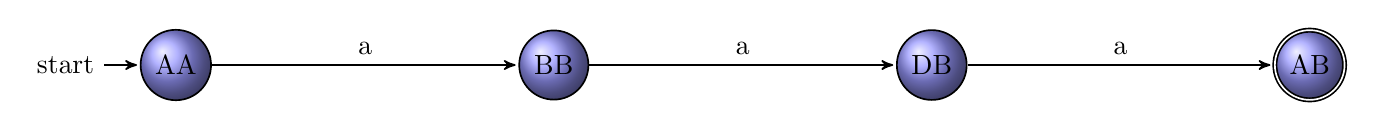
\begin{tikzpicture}[->,>=stealth',shorten >=1pt,auto,node distance=4.8cm, semithick]
\tikzstyle{every state}=[draw=black,text=black, ball color=blue!40]
\node[initial,state] (AA) {AA};
\node[state][right of=AA](BB){BB};
\node[state][right of=BB](DB){DB};
\node[state,accepting][right of=DB](AB){AB};
\path (AA)edge node{a}(BB)
          (BB)edge node{a}(DB)
          (DB)edge node{a}(AB);
\end{tikzpicture} 
\end{center}
\end{figure}

\begin{figure}
\begin{center}
\caption{Q06: $FA_1$}
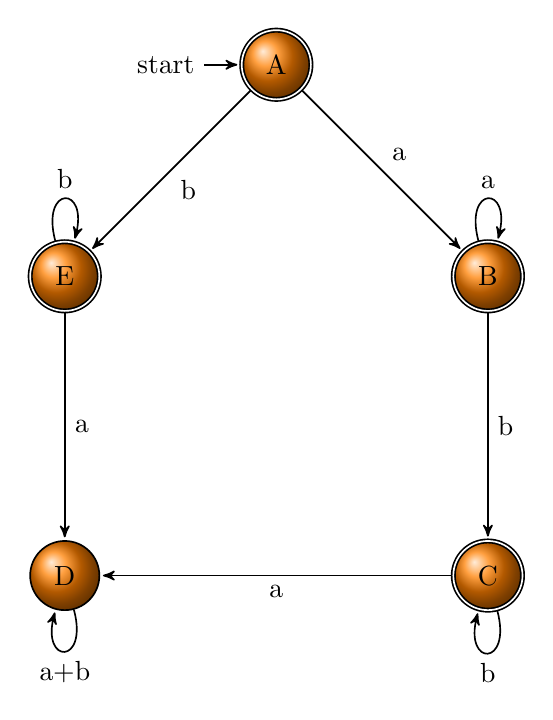
\begin{tikzpicture}[->,>=stealth',shorten >=1pt,auto,node distance=3.8cm, semithick]
\tikzstyle{every state}=[draw=black,text=black, ball color=orange]
\node[initial,state,accepting] (A) {A};
\node[state,accepting][below right of=A](B){B};
\node[state,accepting][below of=B](C){C};
\node[state,accepting][below left of=A](E){E};
\node[state][below of=E](D){D};
\path (A)edge node{a}(B)
              edge node{b}(E)
          (B)edge [loop above]node{a}(B)
              edge node{b}(C)
          (C)edge [loop below]node{b}(C)
              edge node{a}(D)
          (D)edge [loop below]node{a+b}(D)
          (E)edge [loop above]node{b}(E)
              edge node{a}(D);    
\end{tikzpicture} 
\end{center}
\end{figure}

\begin{figure}
\begin{center}
\caption{Q06: $FA_2$}
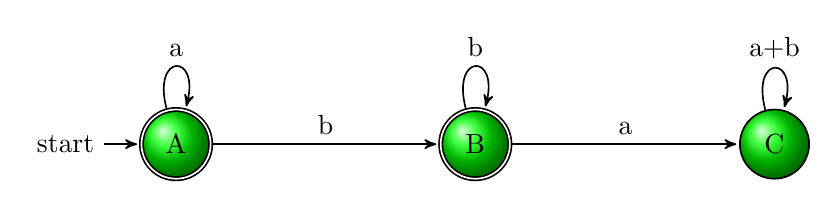
\begin{tikzpicture}[->,>=stealth',shorten >=1pt,auto,node distance=3.8cm, semithick]
\tikzstyle{every state}=[draw=black,text=black, ball color=green]
\node[initial,state,accepting] (A) {A};
\node[state,accepting][right of=A](B){B};
\node[state][right of=B](C){C};
\path (A)edge node{b}(B)
              edge [loop above]node{a}(A)
          (B)edge node{a}(C)
              edge [loop above]node{b}(B)
          (C)edge [loop above]node{a+b}(C);
\end{tikzpicture} 
\end{center}
\end{figure}
\clearpage

\begin{raggedright}
Not acceptable by $L_1$$\bigcap$$L_2$: DC \\*
Acceptable by $L_1$$\bigcap$$L_2$: AA, BA, CB,EB
\end{raggedright}
\begin{figure}
\begin{center}
\caption{Q06: $L_1$$\bigcap$$L_2$}
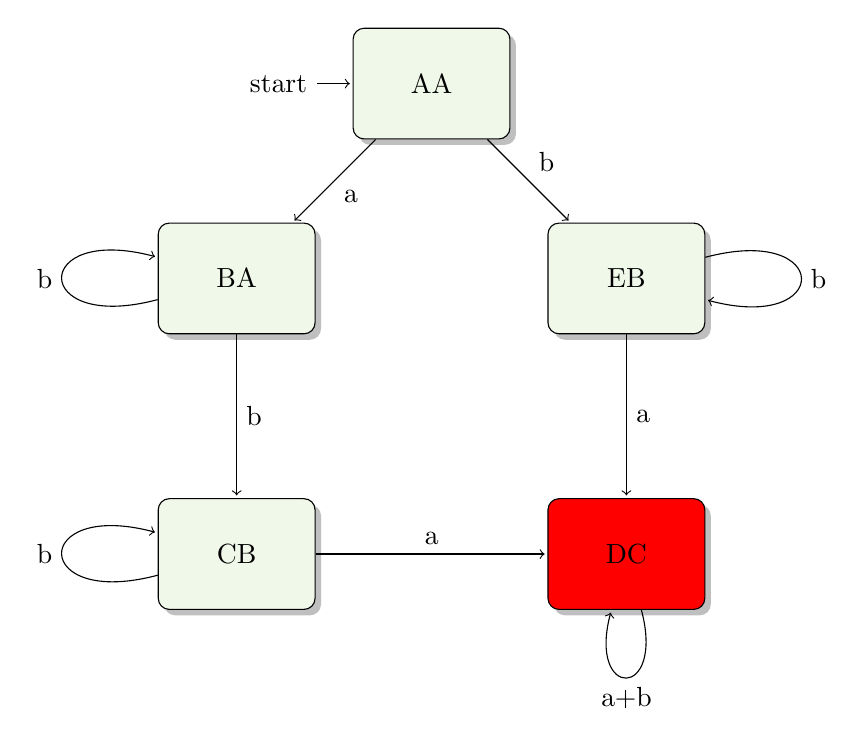
\begin{tikzpicture}[->,shorten >=1pt,node distance=3.5cm,auto]
\tikzstyle{every state} = [rectangle, draw, fill=green!45!brown!10!, text width=5em, text centered, rounded corners, minimum height=4em, drop shadow]
\tikzstyle{Not} = [rectangle, draw, fill=red, text width=5em, text centered, rounded corners, minimum height=4em, drop shadow]
\node[initial,state] (AA){AA};
\node[state][below left of=AA](BA){BA};
\node[state][below right of=AA](EB){EB};
\node[Not][below of=EB](DC){DC};
\node[state][below of=BA](CB){CB};
\path (AA)edge node{a}(BA)
                edge node{b}(EB)
          (BA)edge node{b}(CB)
                edge [loop left]node{b}(BA)
          (CB)edge node{a}(DC)
                edge [loop left]node{b}(CB)
          (EB)edge node{a}(DC)
                edge [loop right]node{b}(EB)
          (DC)edge [loop below]node{a+b}(DC);
                  
\end{tikzpicture}
\end{center}
\end{figure}


\clearpage
The following are equivalent due to the below proofs in Figures 26-31:
\begin{figure}
\begin{center}
\caption{Q07: $FA_1$}
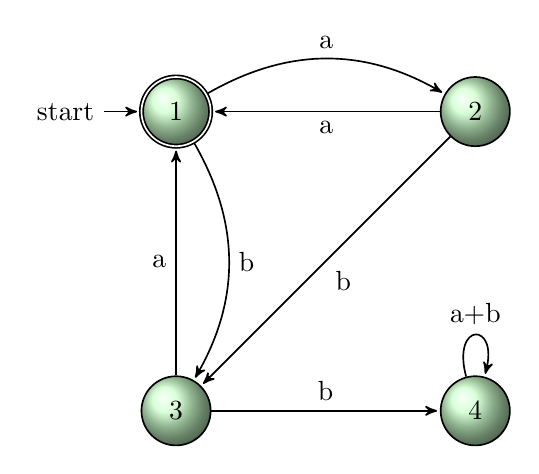
\begin{tikzpicture}[->,>=stealth',shorten >=1pt,auto,node distance=3.8cm, semithick]
\tikzstyle{every state}=[draw=black,text=black, ball color=green!20!]
\node[initial,state,accepting] (1) {1};
\node[state][right of=1](2){2};
\node[state][below of=1](3){3};
\node[state][right of=3](4){4};
\path (1)edge [bend left]node{a}(2)
              edge [bend left]node{b}(3)
          (2)edge node{a}(1)
              edge node{b}(3)
          (3)edge node{a}(1)
              edge node{b}(4)
          (4)edge [loop above]node{a+b}(4);         
\end{tikzpicture} 
\end{center}
\end{figure}

\begin{figure}
\begin{center}
\caption{Q07: $FA_2$}
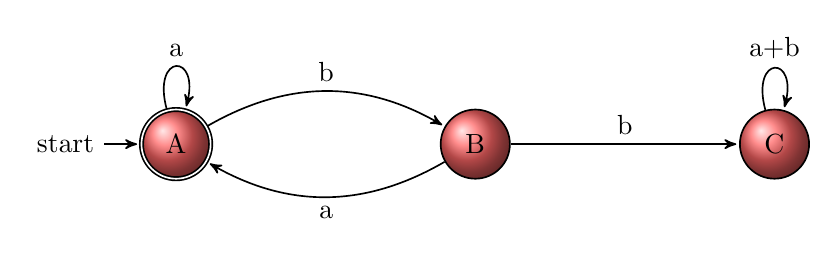
\begin{tikzpicture}[->,>=stealth',shorten >=1pt,auto,node distance=3.8cm, semithick]
\tikzstyle{every state}=[draw=black,text=black, ball color=red!60!]
\node[initial,state,accepting] (A) {A};
\node[state][right of=A](B){B};
\node[state][right of=B](C){C};
\path (A)edge [bend left]node{b}(B)
              edge [loop above]node{a}(A)
          (B)edge [bend left]node{a}(A)
              edge node{b}(C)
          (C)edge [loop above]node{a+b}(C);
       
          
\end{tikzpicture} 
\end{center}
\end{figure}
\clearpage
\begin{figure}
\begin{center}
\caption{Q07: $FA'_1$}
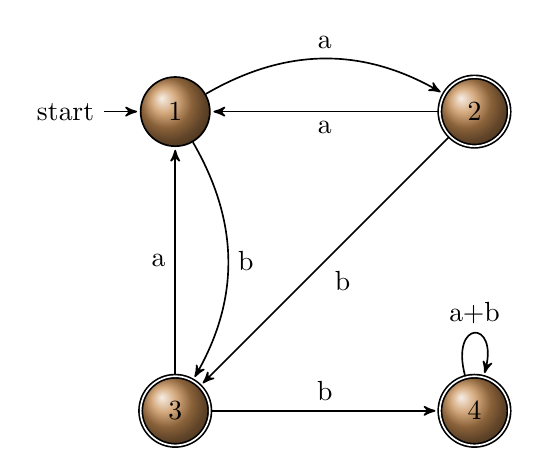
\begin{tikzpicture}[->,>=stealth',shorten >=1pt,auto,node distance=3.8cm, semithick]
\tikzstyle{every state}=[draw=black,text=black, ball color=brown!90!]
\node[initial,state] (1) {1};
\node[state,accepting][right of=1](2){2};
\node[state,accepting][below of=1](3){3};
\node[state,accepting][right of=3](4){4};
\path (1)edge [bend left]node{a}(2)
              edge [bend left]node{b}(3)
          (2)edge node{a}(1)
              edge node{b}(3)
          (3)edge node{a}(1)
              edge node{b}(4)
          (4)edge [loop above]node{a+b}(4);         
\end{tikzpicture} 
\end{center}
\end{figure}

\begin{figure}
\begin{center}
\caption{Q07: $FA_2$}
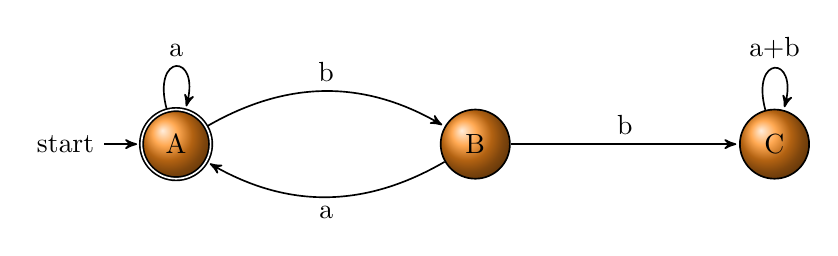
\begin{tikzpicture}[->,>=stealth',shorten >=1pt,auto,node distance=3.8cm, semithick]
\tikzstyle{every state}=[draw=black,text=black, ball color=orange!90!]
\node[initial,state,accepting] (A) {A};
\node[state][right of=A](B){B};
\node[state][right of=B](C){C};
\path (A)edge [bend left]node{b}(B)
              edge [loop above]node{a}(A)
          (B)edge [bend left]node{a}(A)
              edge node{b}(C)
          (C)edge [loop above]node{a+b}(C);       
\end{tikzpicture} 
\end{center}
\end{figure}
\begin{figure}
\begin{center}
\caption{Q07: ($FA\rq{}_1$ + $FA_2$)\rq{} No final states}
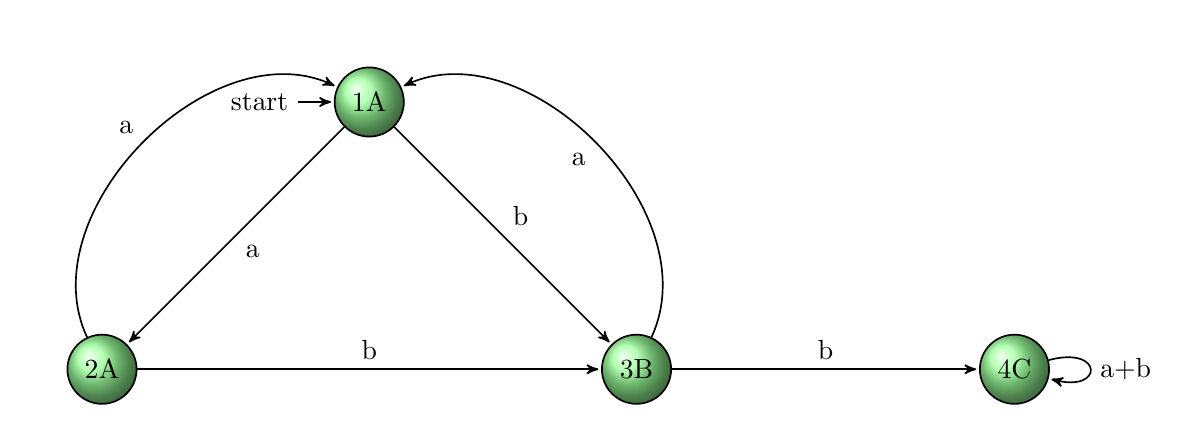
\begin{tikzpicture}[->,>=stealth',shorten >=1pt,auto,node distance=4.8cm, semithick]
\tikzstyle{every state}=[draw=black,text=black, ball color=green!40]
\node[initial,state] (1A) {1A};
\node[state][below left of=1A](2A){2A};
\node[state][below right of=1A](3B){3B};
\node[state][right of=3B](4C){4C};
\path (1A)edge node{a}(2A)
                edge node{b}(3B)
          (2A)edge node{b}(3B)
                edge [bend left=70]node{a}(1A)
          (3B)edge [bend right=70]node{a}(1A)
                edge node{b}(4C)
          (4C)edge [loop right]node{a+b}(4C);        
\end{tikzpicture} 
\end{center}
\end{figure}
\clearpage
\begin{figure}
\begin{center}
\caption{Q07: $FA_1$}
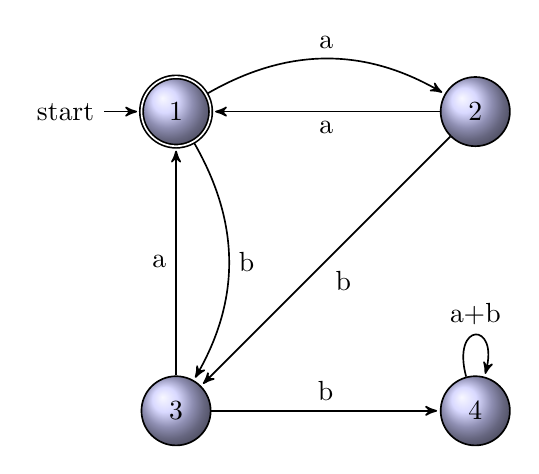
\begin{tikzpicture}[->,>=stealth',shorten >=1pt,auto,node distance=3.8cm, semithick]
\tikzstyle{every state}=[draw=black,text=black, ball color=blue!20!]
\node[initial,state,accepting] (1) {1};
\node[state][right of=1](2){2};
\node[state][below of=1](3){3};
\node[state][right of=3](4){4};
\path (1)edge [bend left]node{a}(2)
              edge [bend left]node{b}(3)
          (2)edge node{a}(1)
              edge node{b}(3)
          (3)edge node{a}(1)
              edge node{b}(4)
          (4)edge [loop above]node{a+b}(4);         
\end{tikzpicture} 
\end{center}
\end{figure}

\begin{figure}
\begin{center}
\caption{Q07: $FA\rq{}_2$}
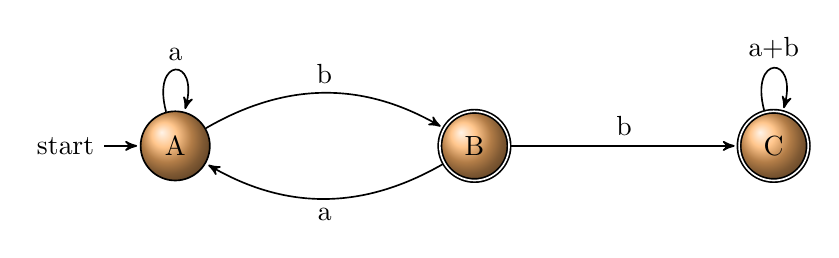
\begin{tikzpicture}[->,>=stealth',shorten >=1pt,auto,node distance=3.8cm, semithick]
\tikzstyle{every state}=[draw=black,text=black, ball color=orange!60!]
\node[initial,state] (A) {A};
\node[state,accepting][right of=A](B){B};
\node[state,accepting][right of=B](C){C};
\path (A)edge [bend left]node{b}(B)
              edge [loop above]node{a}(A)
          (B)edge [bend left]node{a}(A)
              edge node{b}(C)
          (C)edge [loop above]node{a+b}(C);        
\end{tikzpicture} 
\end{center}
\end{figure}

\begin{figure}
\begin{center}
\caption{Q07: ($FA_1$ + $FA\rq{}_2$)\rq{} No final states}
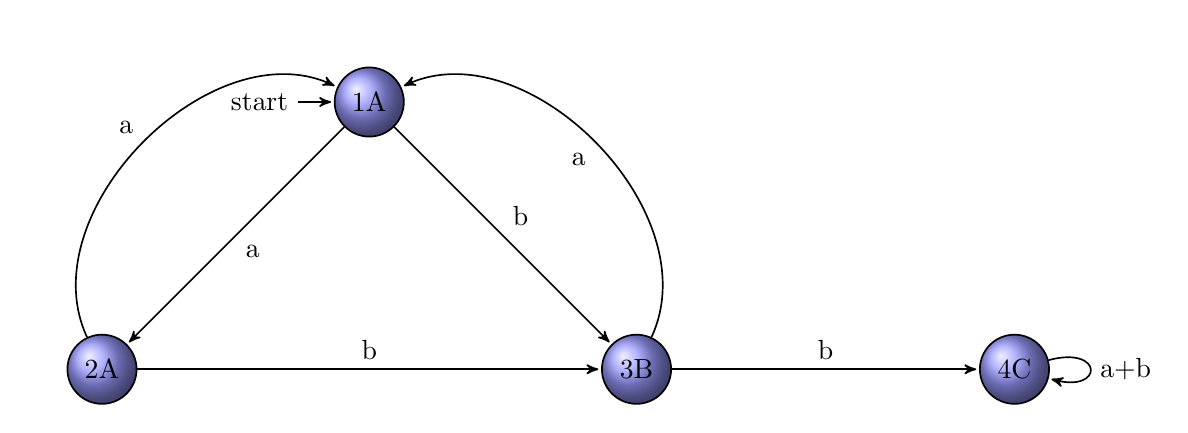
\begin{tikzpicture}[->,>=stealth',shorten >=1pt,auto,node distance=4.8cm, semithick]
\tikzstyle{every state}=[draw=black,text=black, ball color=blue!40]
\node[initial,state] (1A) {1A};
\node[state][below left of=1A](2A){2A};
\node[state][below right of=1A](3B){3B};
\node[state][right of=3B](4C){4C};
\path (1A)edge node{a}(2A)
                edge node{b}(3B)
          (2A)edge node{b}(3B)
                edge [bend left=70]node{a}(1A)
          (3B)edge [bend right=70]node{a}(1A)
                edge node{b}(4C)
          (4C)edge [loop right]node{a+b}(4C);        
\end{tikzpicture} 
\end{center}
\end{figure}

\begin{figure}
\begin{center}
\caption{Q08: $FA_1$}
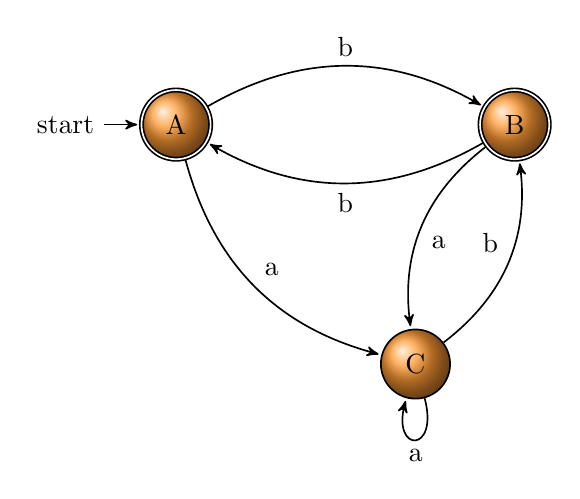
\begin{tikzpicture}[->,>=stealth',shorten >=1pt,auto,node distance=4.3cm, semithick]
\tikzstyle{every state}=[draw=black,text=black, ball color=orange!80!]
\node[initial,state,accepting] (A) {A};
\node[state,accepting][right of=A](B){B};
\node[state][below right of=A](C){C};
\path (A)edge [bend left]node{b}(B)
              edge [bend right]node{a}(C)
          (B)edge [bend left]node{b}(A)
              edge [bend right]node{a}(C)
          (C)edge [bend right]node{b}(B)
              edge[loop below]node{a}(C);
            
\end{tikzpicture} 
\end{center}
\end{figure}

\begin{figure}
\begin{center}
\caption{Q08: $FA_2$}
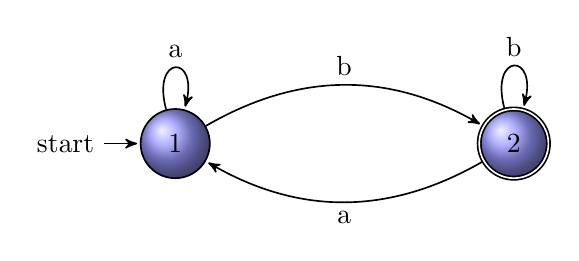
\begin{tikzpicture}[->,>=stealth',shorten >=1pt,auto,node distance=4.3cm, semithick]
\tikzstyle{every state}=[draw=black,text=black, ball color=blue!40!]
\node[initial,state] (1) {1};
\node[accepting,state][right of=1](2){2};
\path (1)edge [bend left]node{b}(2)
             edge [loop above]node{a}(1)
          (2)edge [loop above]node{b}(2)
              edge [bend left]node{a}(1);
\end{tikzpicture} 
\end{center}
\end{figure}

\clearpage
\begin{figure}
\begin{center}
\caption{Q08: $L_1$$\neq$$L_2$}
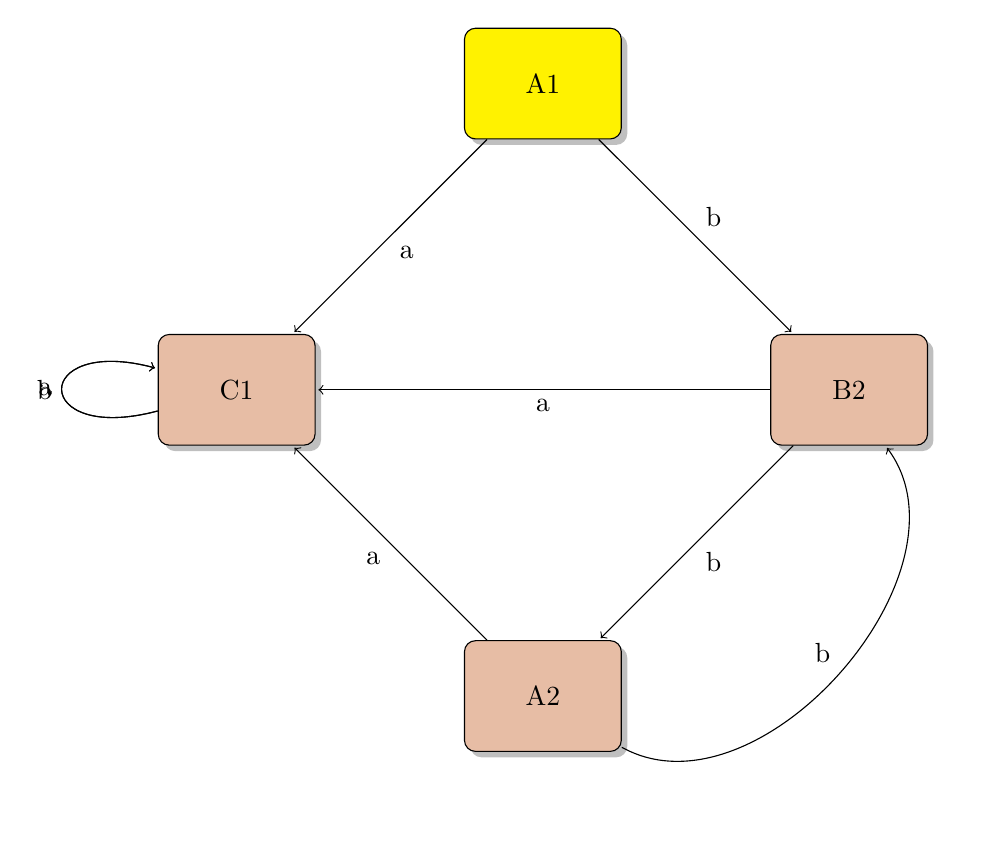
\begin{tikzpicture}[->,shorten >=1pt,node distance=5.5cm,auto]
\tikzstyle{every state} = [rectangle, draw, fill=red!15!brown!45!, text width=5em, text centered, rounded corners, minimum height=4em, drop shadow]
\tikzstyle{Not} = [rectangle, draw, fill=yellow, text width=5em, text centered, rounded corners, minimum height=4em, drop shadow]
\node[Not] (A1){A1};
\node[state][below left of=A1](C1){C1};
\node[state][below right of=A1](B2){B2};
\node[state][below left of=B2](A2){A2};
\path (A1)edge node{a}(C1)
                edge node{b}(B2) 
         (C1)edge [loop left]node{b}(B2)
                edge[loop left]node{a}(C1)
         (B2)edge node{a}(C1)
                edge node{b}(A2)
         (A2)edge node{a}(C1)
                 edge [bend right=78]node{b}(B2);    
\end{tikzpicture}
\end{center}
\end{figure}
\begin{raggedright}
Not acceptable by $L_1$$\bigcap$$L_2$: C1\\*
Acceptable by $L_1$$\bigcap$$L_2$: A2, B2\\*
Acceptable by $L_1$ only: A1, B1\\*
Acceptable by $L_2$ only: C2\\*
Due to A1: $L_1$$\neq$$L_2$
\end{raggedright}

\begin{figure}
\begin{center}
\caption{Q09: $FA_1$}
\begin{tikzpicture}[->,>=stealth',shorten >=1pt,auto,node distance=4.3cm, semithick]
\tikzstyle{every state}=[draw=black,text=black, ball color=red!25!brown!45!]
\node[initial,state] (1) {1};
\node[state][above right of=1](2){2};
\node[state, accepting][right of=A](3){3};
\path (1)edge node{a}(2)
             edge node{b}(3)
         (2)edge [loop above]node{b}(2)
             edge node{a}(3)
         (3)edge [loop right]node{a}(3)
             edge [bend left]node{b}(1);      
\end{tikzpicture} 
\end{center}
\end{figure}

\begin{figure}
\begin{center}
\caption{Q09: $FA_2$}
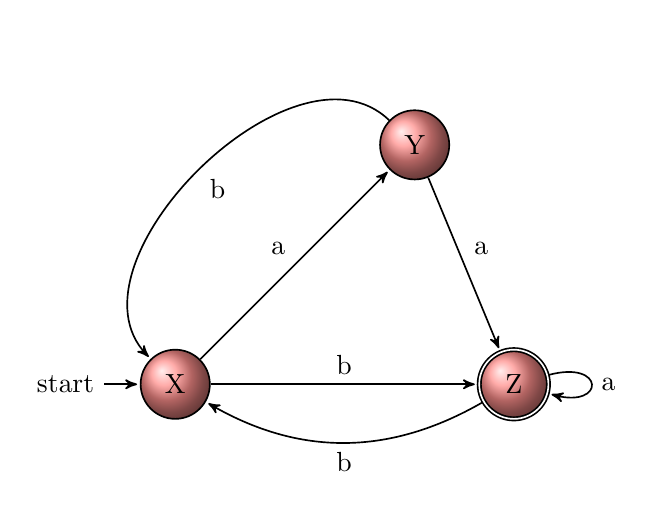
\begin{tikzpicture}[->,>=stealth',shorten >=1pt,auto,node distance=4.3cm, semithick]
\tikzstyle{every state}=[draw=black,text=black, ball color=red!95!orange!45!]
\node[initial,state] (X) {X};
\node[state][above right of=X](Y){Y};
\node[state,accepting][right of=X](Z){Z};
\path (X)edge node{a}(Y)
              edge node{b}(Z)
          (Y)edge[bend right=89]node{b}(X)
              edge node{a}(Z)
          (Z)edge [loop right]node{a}(Z)
              edge [bend left]node{b}(X);
\end{tikzpicture} 
\end{center}
\end{figure}
\clearpage
\begin{figure}
\begin{center}
\caption{Q09: $L_1$$\neq$$L_2$}
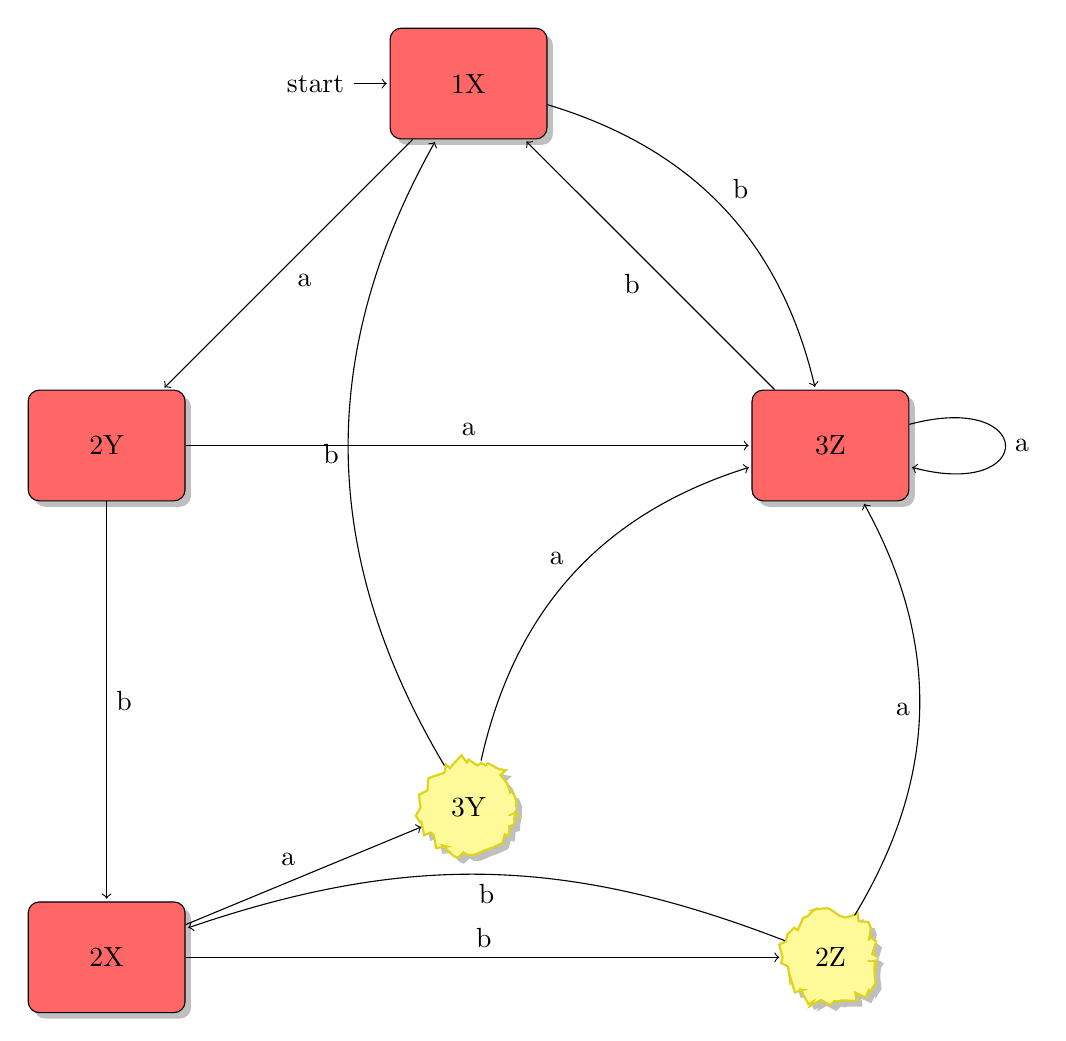
\begin{tikzpicture}[->,shorten >=1pt,node distance=6.5cm,auto]
\tikzstyle{every state} = [rectangle, draw, fill=red!45!red!60!, text width=5em, text centered, rounded corners, minimum height=4em, drop shadow]
\tikzstyle{noise}=[circle,
                                    thick,
                                    minimum size=1.2cm,
                                    draw=yellow!85!black,
                                    fill=yellow!40,
                                    decorate,
                                    drop shadow,
                                    decoration={random steps,
                                                            segment length=2pt,
                                                            amplitude=2pt}]
\node[state,initial] (1X){1X};
\node[state][below left of=1X](2Y){2Y};
\node[state][below right of=1X](3Z){3Z};
\node[state][below of=2Y](2X){2X};
\node[noise][below right of=2Y](3Y){3Y};
\node[noise][below of=3Z](2Z){2Z};
\path (1X)edge node{a}(2Y)
                edge [bend left]node{b}(3Z)
          (2Y)edge node{a}(3Z)
                edge node{b}(2X)
          (3Z)edge [loop right]node{a}(3Z)
                edge node{b}(1X)
          (2X)edge node{a}(3Y)
                 edge node{b}(2Z)
          (3Y)edge [bend left]node{a}(3Z)
                 edge [bend left]node{b}(1X)
          (2Z)edge [bend right]node{a}(3Z)
                edge [bend right=20]node{b}(2X);      
\end{tikzpicture}
\end{center}
\end{figure}


\begin{raggedright}
Not acceptable by $L_1$$\bigcap$$L_2$: 1X,1Y,2X,2Y\\*
Acceptable by $L_1$$\bigcap$$L_2$: 3Z\\*
Acceptable by $L_1$ only: 3X, 3Y\\*
Acceptable by $L_2$ only: 1Z, 2Z\\*
Due to 3Y and 2Z: $L_1$$\neq$$L_2$
\end{raggedright}
\end{document}